\subsection{Implementation} 

hardware, calibration, etc.

\subsection{Results} 
% Table of quantitative results
\paragraph{NYU Depth v2}
The NYU Depth v2 Dataset consists of 249 training and 215 testing scenes of
RGB-D data captured using a Microsoft Kinect. We used a version of DORN
pretrained according to \cite{Fu. et al} as our CNN.
\newpage
\begin{table*}
\begin{center}
\begin{tabular}{lccc|ccc}
  \toprule
    & $\delta^1 \uparrow$ & $\delta^2\uparrow$ & $\delta^3 \uparrow$ & RMSE $\downarrow$ & rel $\downarrow$ & $log_{10} \downarrow$ \\
  \midrule
Eigen et. al. & 0.769 & 0.950 & 0.988 & 0.641 & 0.158 & - \\ 
Laina et. al.&0.811&0.953&0.988&0.573&0.127&0.055 \\
DORN&0.818&0.950&0.982&0.620&0.137&0.063 \\
  DORN (rescaled) & 0.872 & 0.967 & 0.989 & 0.548 & 0.111 & 0.048 \\
Alhashim, Wonka (2019)&0.847&0.973&0.994&0.548(0.461)&0.123&0.053 \\
Alhashim, Wonka (2019) rescaled using GT depth"&0.888&\textbf{0.978}&\textbf{0.995}&\textbf{0.499}(0.409)&\textbf{0.106}&\textbf{0.045} \\
  \midrule
  Ours (raw depth counts) & \textbf{0.899} & 0.970 & 0.990 & 0.529 & 0.199 & 0.055 \\
  Ours (DORN) (intensity/falloff) & 0.835 & 0.953 & 0.984 & 0.521 & 0.129 & 0.060 \\
  Ours (DenseDepth) (intensity/falloff) & 0.867 & 0.974 & 0.994 & 0.445 & 0.114 & 0.050 \\
  \bottomrule
\end{tabular} 
\end{center}
\caption{Results on the NYU Depth v2 test set \cite{nyudepth}.}
\end{table*}
%%%
\begin{table*}
\begin{center}
\begin{tabular}{lccc|ccc}
  \toprule
    & $\delta^1 \uparrow$ & $\delta^2\uparrow$ & $\delta^3 \uparrow$ & RMSE $\downarrow$ & rel $\downarrow$ & $log_{10} \downarrow$ \\
  \midrule
  DORN (cite)&0.846&0.954&0.983&0.501&0.120&0.053 \\
DenseNet(cite))&0.847&0.973&0.994&0.461&0.123&0.054 \\
  \midrule
  DORN (rescaled) & 0.872 & 0.967 & 0.989 & 0.548 & 0.111 & 0.048 \\
  DORN (Wass) & 0.847 & 0.953 & 0.983 & 0.499 & 0.117 & 0.053 \\
  DORN (Histogram Matching) & 0.902 & 0.973 & 0.991 & 0.424 & 0.099 & 0.042 \\
  DenseNet (rescaled) &0.888 & 0.978&0.995&0.409&0.106&0.045 \\
  DenseNet (Wass) & - & - & - & - & - & - \\ 
  DenseNet (Histogram Matching) &\textbf{0.930} &\textbf{0.984}&\textbf{0.995}&\textbf{0.338}&\textbf{0.080}&\textbf{0.034}\\
  \midrule
  DORN (Median SPAD Rescaling) & - & - & - & - & - & - \\
  DORN + Wasserstein (intensity/falloff) & 0.835 & 0.953 & 0.984 & 0.521 & 0.129 & 0.060 \\
  DenseDepth (Median SPAD Rescaling) & - & - & - & - & - & - \\
  DenseDepth + Wasserstein (intensity/falloff) & 0.867 & 0.974 & 0.994 & 0.445 & 0.114 & 0.050 \\
  \midrule
  \bottomrule
\end{tabular} 
\end{center}
\caption{Results on the NYU Depth v2 test set \cite{nyudepth}.}
\end{table*}

\begin{figure}
  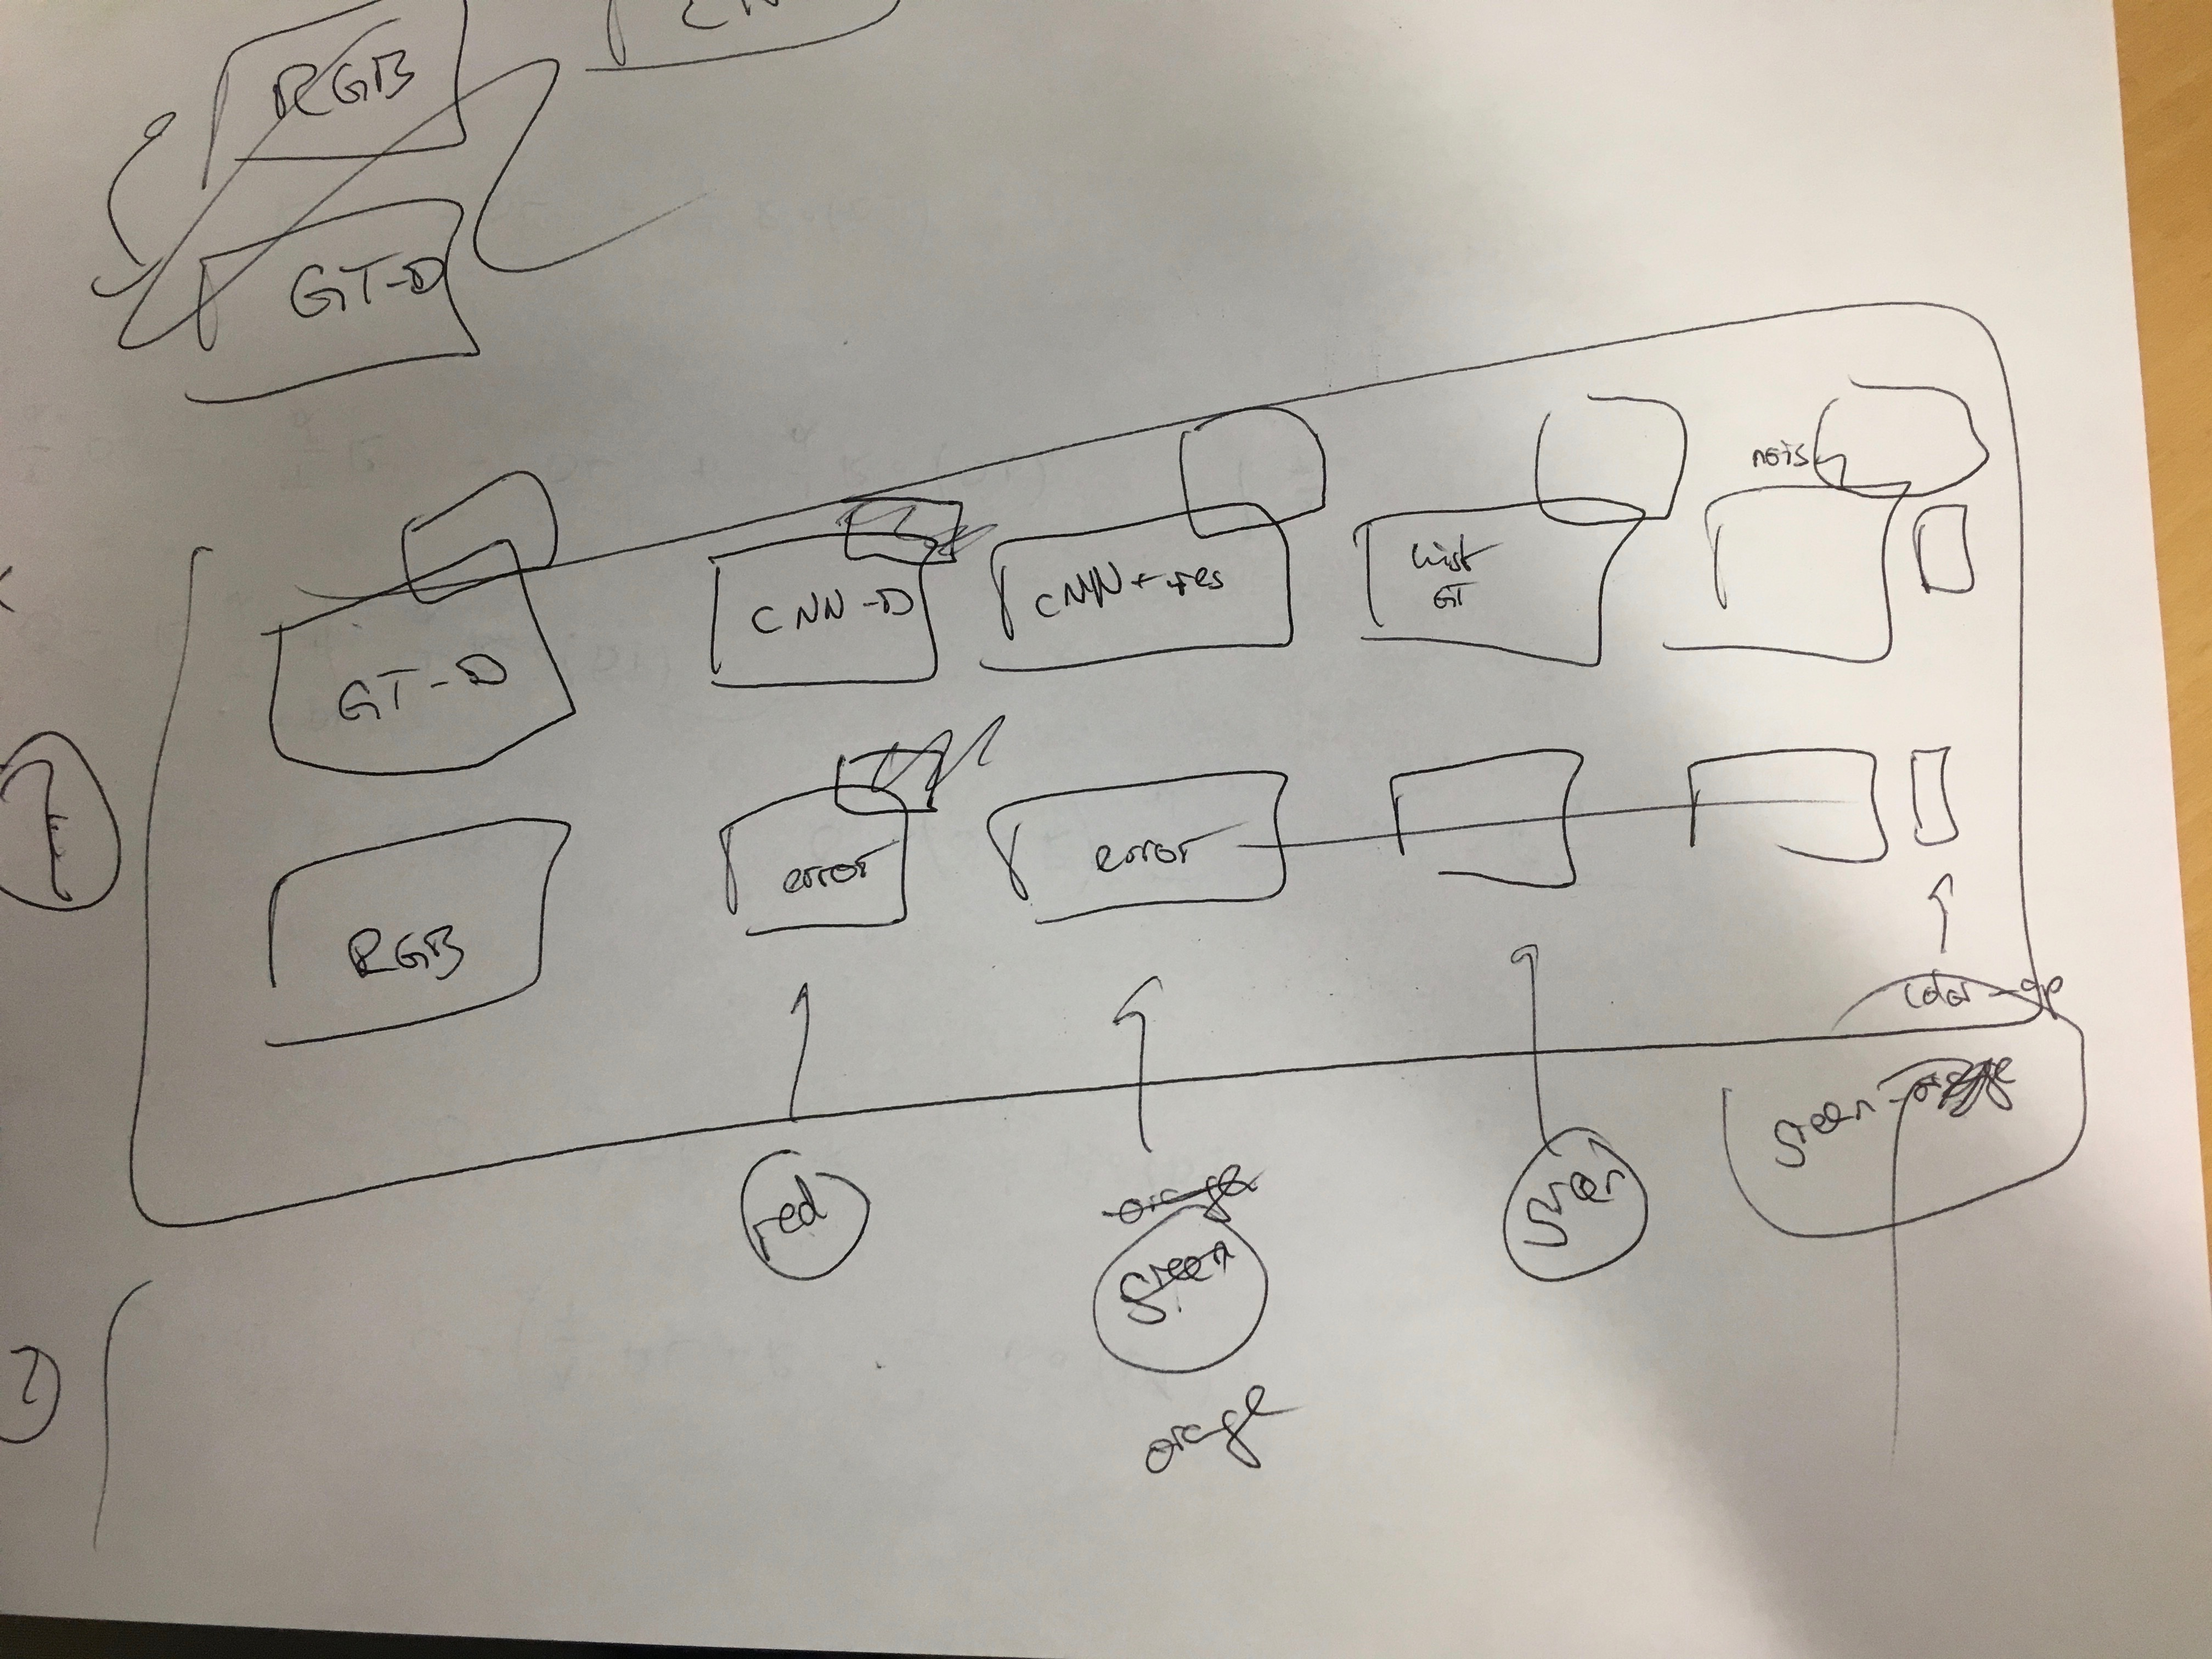
\includegraphics[width=\textwidth/2]{sections/figures/comparison.jpeg}
  \caption{\textbf{Comparing our results with other methods}}
\end{figure}
% Table of qualitative results
%\begin{table*}
%  \begin{center}
%    \begin{tabularx}{\linewidth}{*{5}{X}}
%      RGB & Ground Truth & CNN & CNN + Raw Histogram & CNN + Albedo/Falloff \\
%        \includegraphics[width=\textwidth/6-5pt]{sections/figures/comparison_table/rgb_0.png} &
%      \includegraphics[width=\textwidth/6-5pt]{sections/figures/comparison_table/gt_0.png} &
%      \includegraphics[width=\textwidth/6-5pt]{sections/figures/comparison_table/cnn_diff_0.png} &
%      \includegraphics[width=\textwidth/6-5pt]{sections/figures/comparison_table/cnn_rawhist_diff_0.png} &
%      \includegraphics[width=\textwidth/6-5pt]{sections/figures/comparison_table/cnn_hist_diff_0.png} \\ 
%  & & RMSE = 0.462, WAS = 34.615 & RMSE = 0.263, WAS = 11.906 & RMSE = 0.271, WAS = 13.149 \\
%        \includegraphics[width=\textwidth/6-5pt]{sections/figures/comparison_table/rgb_1.png} &
%      \includegraphics[width=\textwidth/6-5pt]{sections/figures/comparison_table/gt_1.png} &
%      \includegraphics[width=\textwidth/6-5pt]{sections/figures/comparison_table/cnn_diff_1.png} &
%      \includegraphics[width=\textwidth/6-5pt]{sections/figures/comparison_table/cnn_rawhist_diff_1.png} &
%      \includegraphics[width=\textwidth/6-5pt]{sections/figures/comparison_table/cnn_hist_diff_1.png} \\ 
%  & & RMSE = 0.463, WAS = 9.620 & RMSE = 0.290, WAS = 5.765 & RMSE = 0.372, WAS = 3.854 \\
%      \includegraphics[width=\textwidth/6-5pt]{sections/figures/comparison_table/rgb_2.png} &
%      \includegraphics[width=\textwidth/6-5pt]{sections/figures/comparison_table/gt_2.png} &
%      \includegraphics[width=\textwidth/6-5pt]{sections/figures/comparison_table/cnn_diff_2.png} &
%      \includegraphics[width=\textwidth/6-5pt]{sections/figures/comparison_table/cnn_rawhist_diff_2.png} &
%      \includegraphics[width=\textwidth/6-5pt]{sections/figures/comparison_table/cnn_hist_diff_2.png} \\ 
%    & & RMSE = 0.667, WAS = 72.725 & RMSE = 0.471, WAS = 43.348 & RMSE = 0.584, WAS = 52.787 \\
%        \includegraphics[width=\textwidth/6-5pt]{sections/figures/comparison_table/rgb_3.png} &
%      \includegraphics[width=\textwidth/6-5pt]{sections/figures/comparison_table/gt_3.png} &
%      \includegraphics[width=\textwidth/6-5pt]{sections/figures/comparison_table/cnn_diff_3.png} &
%      \includegraphics[width=\textwidth/6-5pt]{sections/figures/comparison_table/cnn_rawhist_diff_3.png} &
%      \includegraphics[width=\textwidth/6-5pt]{sections/figures/comparison_table/cnn_hist_diff_3.png} \\ 
%  & & RMSE = 1.486, WAS = 31.845 & RMSE = 1.189, WAS = 21.868 & RMSE = 1.844, WAS = 121.540 \\
%    \end{tabularx}
%  \end{center}
%  \caption{\textbf{NYU Depth v2} Qualitative comparison of the raw output of
%    DORN, the corrected depth map when the ground-truth depth histogram is used,
%    and the corrected depth when the simulated SPAD measurements are used.}
%\end{table*}
\begin{itemize}
\item Overlay spad histograms?
\item Show RMSE/delta1/etc.
\item Show colorbars in the last column.
\item Show inset squares and then show the zoomed regions in more detail?
\end{itemize}


